\documentclass[12pt,letterpaper]{article}

\usepackage[margin=0.75in]{geometry}
\usepackage{amsmath,amssymb}
\usepackage{enumitem}
\usepackage{environ}
\usepackage{tikz}

\pagestyle{plain}
\setlength{\parindent}{0pt}
\setlength{\parskip}{0.5em}
\setlength{\emergencystretch}{2em}

% Solutions are hidden unless \showsolutions is defined; midterm2_key.tex does
% this and then inputs this file, producing the answer key as a separate PDF.
\newif\ifsolutions
\ifdefined\showsolutions\solutionstrue\fi

\NewEnviron{solution}{%
  \ifsolutions
    \par{\color{blue!55!black}\textbf{Solution.} \BODY\par}%
  \fi}

\newcommand{\points}[1]{(#1 points)}
\newcommand{\workspace}{\vfill\newpage}

\begin{document}

\thispagestyle{empty}

\begin{center}
  {\large\bfseries MATH 15200: Calculus II}\\
  {\large\bfseries Midterm 2}\\[0.3em]
  Thursday, November 19, 2026
\end{center}

\vspace{0.25em}
\hrule
\vspace{1.5em}

\textbf{Name:} \rule{4in}{0.4pt}

\ifsolutions
  \begin{center}
    {\color{blue!55!black}\large\bfseries ANSWER KEY}
  \end{center}
\fi

\vspace{0.8em}

\textbf{Instructions.} You have 80 minutes. No notes, books, calculators,
phones, or other electronic devices are allowed. Show all of your work and
justify your answers; a correct answer without supporting work may not receive
full credit. Give exact answers (such as $\tfrac{\sqrt{2}}{3}$ or $5\pi$), not
decimal approximations. The last page is extra space. If you run out of room
on a problem, you may continue your answer there; if you do, write on that
problem's page that your answer continues on the last page, and label your
work on the last page with the problem number.

\vspace{0.8em}

\begin{center}\setlength{\tabcolsep}{40pt}
\textbf{Trigonometric identities:} \\[10pt]
\renewcommand{\arraystretch}{1.5}
\begin{tabular}{ll}
  $\bullet \sin^2x+\cos^2x=1$ & $\bullet \tan^2x+1=\sec^2x$\\
  $\bullet \sin2x=2\sin x\cos x$ & $\bullet \cos2x=2\cos^2x-1=1-2\sin^2x$
\end{tabular}
\end{center}

\vfill

\begin{center}
  \renewcommand{\arraystretch}{1.5}
  \begin{tabular}{|c|c|p{1in}|}
    \hline
    \textbf{Problem} & \textbf{Points} & \textbf{Score} \\
    \hline
    1 & 15 & \\ \hline
    2 & 15 & \\ \hline
    3 & 20 & \\ \hline
    4 & 15 & \\ \hline
    5 & 15 & \\ \hline
    6 & 20 (+5) & \\ \hline
    \textbf{Total} & 100 & \\ \hline
  \end{tabular}
\end{center}

\vfill
\newpage

\begin{enumerate}[label=\textbf{\arabic*.},leftmargin=2em]
  \item \points{15}
    \begin{enumerate}[label=(\alph*)]
      \item \points{10} Use the definition of the derivative of $\ln x$ at
        $x=1$ to show that
        \[
          \lim_{x\to 0}\frac{\ln(1+x)}{x}=1.
        \]

        \begin{solution}
          Let $g(x)=\ln x$. Then $g'(x)=\frac1x$, so $g'(1)=1$. By the
          definition of the derivative, and since $\ln 1=0$,
          \[
            1=g'(1)=\lim_{x\to0}\frac{g(1+x)-g(1)}{x}
             =\lim_{x\to0}\frac{\ln(1+x)-\ln 1}{x}
             =\lim_{x\to0}\frac{\ln(1+x)}{x}.
          \]
        \end{solution}
        \vfill

      \item \points{5} Use part (a) to show that
        \[
          \lim_{x\to 0}\,(1+x)^{1/x}=e.
        \]

        \begin{solution}
          For $x>-1$ with $x\neq0$,
          \[
            (1+x)^{1/x}=e^{\frac1x\ln(1+x)}=e^{\ln(1+x)/x}.
          \]
          By part (a), the exponent tends to $1$ as $x\to0$. Since the
          exponential function is continuous,
          \[
            \lim_{x\to0}(1+x)^{1/x}
            =e^{\lim_{x\to0}\ln(1+x)/x}=e^1=e.
          \]
        \end{solution}
        \vfill
    \end{enumerate}
    \newpage

  \item \points{15}
    Let $f(x)=x^5+2x^3+x$.
    \begin{enumerate}[label=(\alph*)]
      \item \points{10} Find $(f^{-1})'(4)$.

        \begin{solution}
          Since $f(1)=1+2+1=4$, we have $f^{-1}(4)=1$. Also
          $f'(1)=5+6+1=12$. Hence
          \[
            (f^{-1})'(4)=\frac{1}{f'\bigl(f^{-1}(4)\bigr)}
              =\frac{1}{f'(1)}=\frac{1}{12}.
          \]
        \end{solution}
        \vfill

      \item \points{5} Find an equation of the tangent line to the graph of
        $y=f^{-1}(x)$ at $x=4$.

        \begin{solution}
          The point of tangency is $\bigl(4,f^{-1}(4)\bigr)=(4,1)$ and the
          slope is $\tfrac1{12}$, so the tangent line is
          \[
            y=1+\frac{1}{12}(x-4),\quad\text{that is,}\quad
            y=\frac{x}{12}+\frac23.
          \]
        \end{solution}
        \vfill
    \end{enumerate}
    \newpage

  \item \points{20}
    Evaluate the following integrals.
    \begin{enumerate}[label=(\alph*)]
      \item \points{10}\quad
        $\displaystyle\int_0^1\arctan x\,dx$

        \begin{solution}
          Integrate by parts with $u=\arctan x$ and $dv=dx$, so
          $du=\dfrac{dx}{1+x^2}$ and $v=x$:
          \[
            \int_0^1\arctan x\,dx
            =\Bigl[x\arctan x\Bigr]_0^1-\int_0^1\frac{x}{1+x^2}\,dx
            =\frac\pi4-\Bigl[\frac12\ln\bigl(1+x^2\bigr)\Bigr]_0^1
            =\frac\pi4-\frac12\ln 2,
          \]
          where the last integral uses the substitution $w=1+x^2$.
        \end{solution}
        \vfill

      \item \points{10}\quad
        $\displaystyle\int_1^{e^{\pi}}\sin(\ln x)\,dx$

        \begin{solution}
          Let $I=\int_1^{e^\pi}\sin(\ln x)\,dx$. Integrate by parts with
          $u=\sin(\ln x)$ and $dv=dx$, so $du=\cos(\ln x)\,\frac{dx}{x}$ and
          $v=x$. Since $\sin(\ln e^\pi)=\sin\pi=0$ and $\sin(\ln 1)=0$,
          \[
            I=\Bigl[x\sin(\ln x)\Bigr]_1^{e^\pi}-\int_1^{e^\pi}\cos(\ln x)\,dx
             =-\int_1^{e^\pi}\cos(\ln x)\,dx.
          \]
          Integrate by parts again with $u=\cos(\ln x)$ and $dv=dx$, so
          $du=-\sin(\ln x)\,\frac{dx}{x}$ and $v=x$. Since
          $\cos(\ln e^\pi)=-1$ and $\cos(\ln1)=1$,
          \[
            \int_1^{e^\pi}\cos(\ln x)\,dx
            =\Bigl[x\cos(\ln x)\Bigr]_1^{e^\pi}+\int_1^{e^\pi}\sin(\ln x)\,dx
            =-e^\pi-1+I.
          \]
          Hence $I=e^\pi+1-I$, so
          \[
            I=\frac{e^\pi+1}{2}.
          \]
          (Alternatively, substituting $x=e^t$ gives
          $I=\int_0^\pi e^t\sin t\,dt$, which can be done by integrating by
          parts twice.)
        \end{solution}
        \vfill
    \end{enumerate}
    \newpage

  \item \points{15}
    \begin{enumerate}[label=(\alph*)]
      \item \points{10} Let $n\ge1$ be an integer. Prove that for $x>0$,
        \[
          \int(\ln x)^n\,dx=x(\ln x)^n-n\int(\ln x)^{n-1}\,dx.
        \]

        \begin{solution}
          Integrate by parts with $u=(\ln x)^n$ and $dv=dx$. By the chain
          rule, $du=n(\ln x)^{n-1}\cdot\frac1x\,dx$, and $v=x$. Hence
          \[
            \int(\ln x)^n\,dx
            =x(\ln x)^n-\int x\cdot n(\ln x)^{n-1}\cdot\frac1x\,dx
            =x(\ln x)^n-n\int(\ln x)^{n-1}\,dx.
          \]
        \end{solution}
        \vfill

      \item \points{5} Compute $\displaystyle\int_1^e(\ln x)^2\,dx$.

        \begin{solution}
          Let $I_n=\int_1^e(\ln x)^n\,dx$. For $n\ge1$, part (a) gives
          \[
            I_n=\Bigl[x(\ln x)^n\Bigr]_1^e-nI_{n-1}=e-nI_{n-1},
          \]
          since $\ln e=1$ and $\ln 1=0$. Starting from
          $I_0=\int_1^e dx=e-1$,
          \[
            I_1=e-(e-1)=1,\qquad I_2=e-2\cdot1=e-2.
          \]
          Hence $\displaystyle\int_1^e(\ln x)^2\,dx=e-2$.
        \end{solution}
        \vfill
    \end{enumerate}
    \newpage

  \item \points{15}
    Evaluate
    \[
      \int\frac{dx}{\bigl(x^2+9\bigr)^{3/2}}.
    \]

    \begin{solution}
      Let $x=3\tan\theta$ with $-\frac\pi2<\theta<\frac\pi2$, so
      $dx=3\sec^2\theta\,d\theta$. Then
      $x^2+9=9\tan^2\theta+9=9\sec^2\theta$, and since $\sec\theta>0$ on
      this interval, $\bigl(x^2+9\bigr)^{3/2}=27\sec^3\theta$. Hence
      \[
        \int\frac{dx}{\bigl(x^2+9\bigr)^{3/2}}
        =\int\frac{3\sec^2\theta}{27\sec^3\theta}\,d\theta
        =\frac19\int\cos\theta\,d\theta
        =\frac19\sin\theta+C.
      \]
      Since $\tan\theta=\frac x3$, a right triangle with legs $x$ and $3$
      and hypotenuse $\sqrt{x^2+9}$ gives
      $\sin\theta=x/\sqrt{x^2+9}$. Therefore
      \[
        \int\frac{dx}{\bigl(x^2+9\bigr)^{3/2}}=\frac{x}{9\sqrt{x^2+9}}+C.
      \]
      (Check: $\dfrac{d}{dx}\dfrac{x}{\sqrt{x^2+9}}
      =\dfrac{(x^2+9)-x^2}{(x^2+9)^{3/2}}=\dfrac{9}{(x^2+9)^{3/2}}$.)
    \end{solution}
    \workspace

  \item (20 points, plus 5 points extra credit)
    Let $R$ be the region bounded by the curve $y=\dfrac{1}{1+x^2}$, the
    $x$-axis, the $y$-axis, and the line $x=1$ (see the figure).

    \begin{center}
      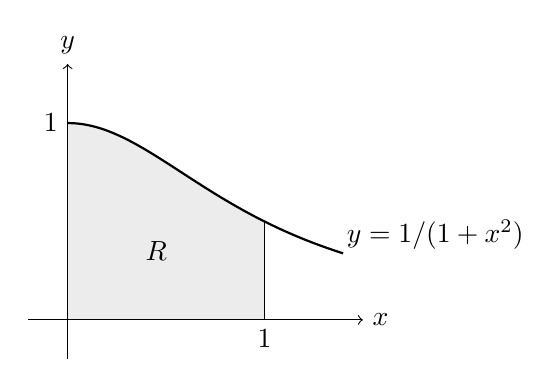
\begin{tikzpicture}[scale=2.5,
          declare function={g(\x)=1/(1+\x*\x);}]
        \fill[gray!15] (0,0) -- plot[domain=0:1, samples=60] (\x,{g(\x)})
          -- (1,0) -- cycle;
        \draw[->] (-0.2,0) -- (1.5,0) node[right] {$x$};
        \draw[->] (0,-0.2) -- (0,1.3) node[above] {$y$};
        \draw[thick] plot[domain=0:1.4, samples=80] (\x,{g(\x)})
          node[above right, inner sep=1pt] {$y=1/(1+x^2)$};
        \draw (1,0) -- (1,{g(1)});
        \node[below] at (1,0) {$1$};
        \node[left] at (0,1) {$1$};
        \node at (0.45,0.35) {$R$};
      \end{tikzpicture}
    \end{center}

    \begin{enumerate}[label=(\alph*)]
      \item \points{20} Find the volume of the solid formed by revolving $R$
        about the $x$-axis.

        \begin{solution}
          By the disk method,
          \[
            V=\pi\int_0^1\Bigl(\frac{1}{1+x^2}\Bigr)^2dx
             =\pi\int_0^1\frac{dx}{\bigl(1+x^2\bigr)^2}.
          \]
          Let $x=\tan\theta$, so $dx=\sec^2\theta\,d\theta$ and
          $1+x^2=\sec^2\theta$; when $x=0$, $\theta=0$, and when $x=1$,
          $\theta=\frac\pi4$. Then
          \begin{align*}
            \int_0^1\frac{dx}{\bigl(1+x^2\bigr)^2}
            &=\int_0^{\pi/4}\frac{\sec^2\theta}{\sec^4\theta}\,d\theta
             =\int_0^{\pi/4}\cos^2\theta\,d\theta
             =\frac12\int_0^{\pi/4}\bigl(1+\cos2\theta\bigr)\,d\theta\\
            &=\frac12\Bigl[\theta+\frac12\sin2\theta\Bigr]_0^{\pi/4}
             =\frac12\Bigl(\frac\pi4+\frac12\Bigr)
             =\frac\pi8+\frac14.
          \end{align*}
          Hence
          \[
            V=\pi\Bigl(\frac\pi8+\frac14\Bigr)=\frac{\pi^2}{8}+\frac{\pi}{4}.
          \]
        \end{solution}
        % Twice the stretch of the \vfill after part (b), so part (a) gets
        % about two thirds of the remaining space on the page.
        \vspace{\stretch{2}}

      \item (5 points, extra credit) What if we removed the $x$-bounds entirely?
      Compute the volume of the solid given by revolving the {\it entire} 
      region bounded between $y = 1/(1 + x^2)$ and $y=0$ about the $x$-axis.

        \begin{solution}
          The region is unbounded, so we interpret the volume as
          $\lim_{b\to\infty}V(b)$, where $V(b)$ is the volume obtained by
          revolving the part of the region with $-b\le x\le b$. Since
          $1/(1+x^2)$ is even, $V(b)$ is twice the volume from
          $0\le x\le b$. As in part (a), with $x=\tan\theta$ and
          $\theta_b=\arctan b$,
          \[
            V(b)=2\pi\int_0^b\frac{dx}{\bigl(1+x^2\bigr)^2}
             =2\pi\int_0^{\theta_b}\cos^2\theta\,d\theta
             =\pi\Bigl[\theta+\frac12\sin2\theta\Bigr]_0^{\theta_b}
             =\pi\Bigl(\theta_b+\sin\theta_b\cos\theta_b\Bigr).
          \]
          As $b\to\infty$, $\theta_b=\arctan b\to\frac\pi2$, so
          $\sin\theta_b\cos\theta_b\to\sin\frac\pi2\cos\frac\pi2=0$. Hence
          the volume is
          \[
            \lim_{b\to\infty}V(b)=\pi\cdot\frac\pi2=\frac{\pi^2}{2}.
          \]
          (Equivalently, $\sin\theta_b\cos\theta_b=\dfrac{b}{1+b^2}$, so
          $V(b)=\pi\Bigl(\arctan b+\dfrac{b}{1+b^2}\Bigr)$. A student who
          revolves only the part with $x\ge0$ gets $\frac{\pi^2}{4}$.)
        \end{solution}
        \vfill
    \end{enumerate}
    \newpage
\end{enumerate}

\begin{center}
  {\Large\bfseries Extra Space}\\[0.3em]
  \noindent\rule{\linewidth}{0.4pt}
\end{center}

\end{document}
